\documentclass{article}
\usepackage{tikz}
\usetikzlibrary{shapes.geometric, arrows}

\begin{document}

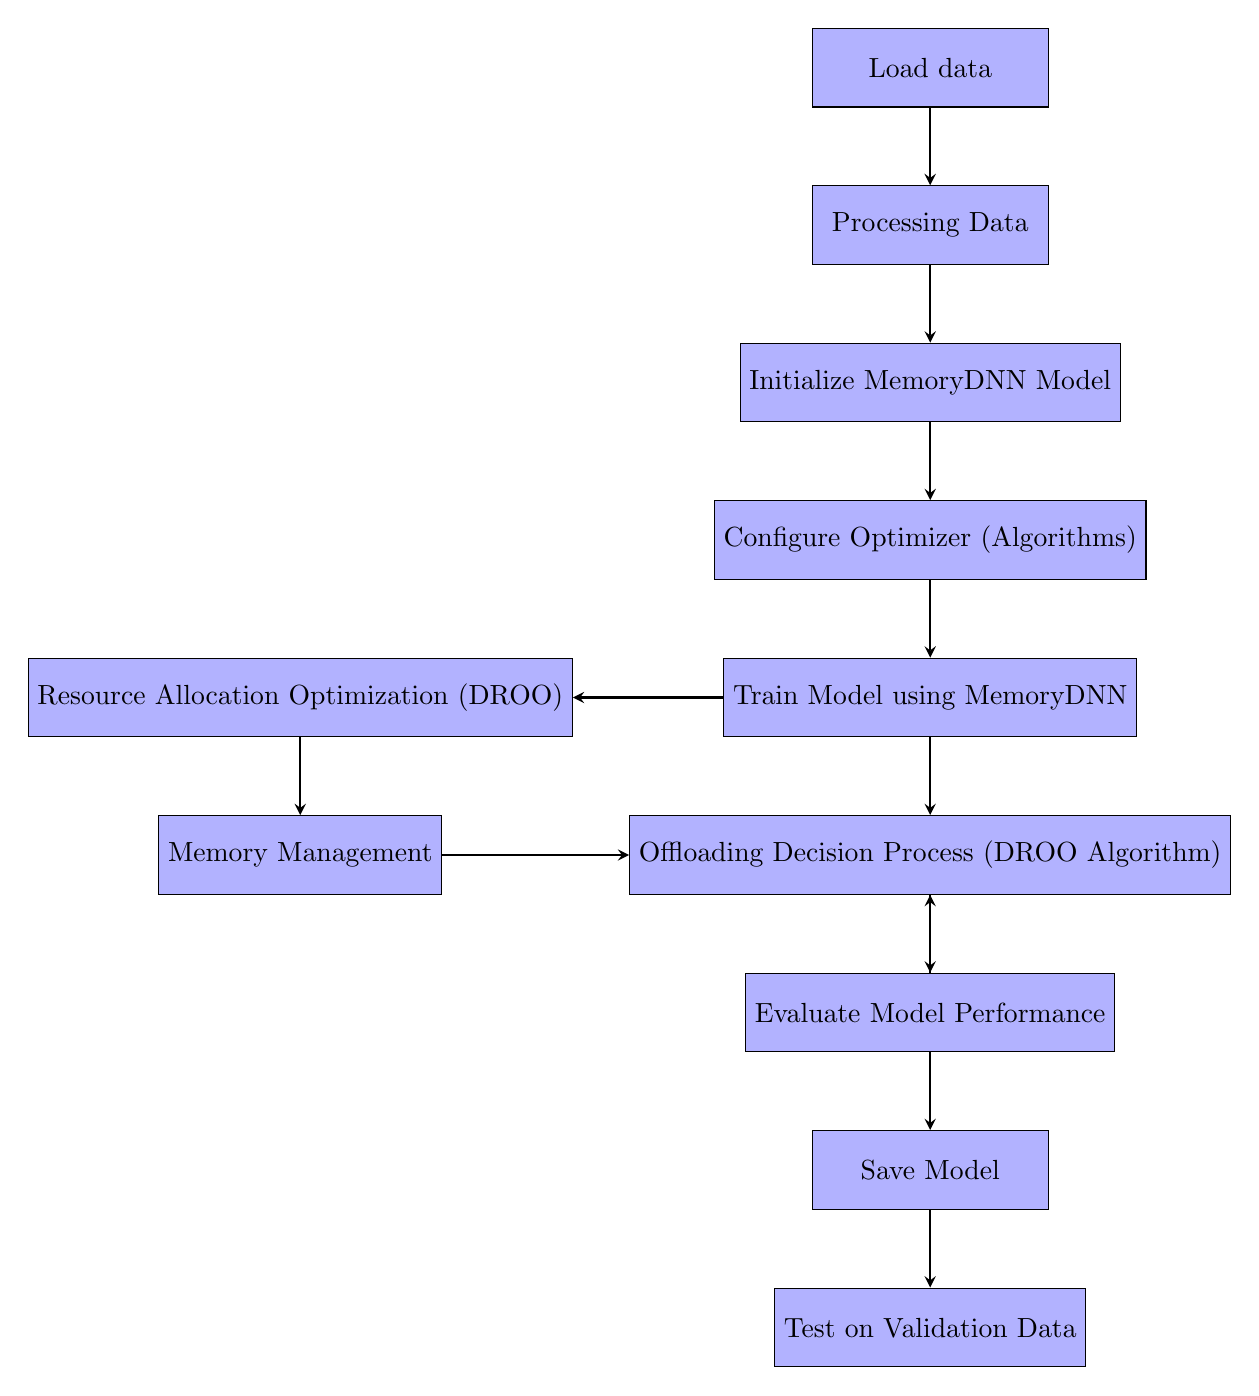
\begin{tikzpicture}[node distance=2cm]

% Define block styles
\tikzstyle{block} = [rectangle, draw, fill=blue!30, text centered, minimum height=1cm, minimum width=3cm]
\tikzstyle{arrow} = [thick,->,>=stealth]

% Nodes
\node (load) [block] {Load data};
\node (process) [block, below of=load] {Processing Data};
\node (init) [block, below of=process] {Initialize MemoryDNN Model};
\node (optimizer) [block, below of=init] {Configure Optimizer (Algorithms)};
\node (train) [block, below of=optimizer] {Train Model using MemoryDNN};
\node (resource) [block, left of=train, xshift=-6cm] {Resource Allocation Optimization (DROO)};
\node (offload) [block, below of=train] {Offloading Decision Process (DROO Algorithm)};
\node (memory) [block, left of=offload, xshift=-6cm] {Memory Management};
\node (evaluate) [block, below of=offload] {Evaluate Model Performance};
\node (save) [block, below of=evaluate] {Save Model};
\node (test) [block, below of=save] {Test on Validation Data};

% Arrows
\draw [arrow] (load) -- (process);
\draw [arrow] (process) -- (init);
\draw [arrow] (init) -- (optimizer);
\draw [arrow] (optimizer) -- (train);
\draw [arrow] (train) -- (offload);
\draw [arrow] (train) -- (resource);
\draw [arrow] (resource) -- (memory);
\draw [arrow] (memory) -- (offload);
\draw [arrow] (offload) -- (evaluate);
\draw [arrow] (evaluate) -- (save);
\draw [arrow] (save) -- (test);

% Feedback loop
\draw [arrow, dashed] (evaluate) -- (offload);

\end{tikzpicture}

\end{document}
